\subsection{Der Eventbus}

Der Eventbus stellt für Softwarekomponenten die Möglichkeit bereit, Ereignisse untereinander auszutauschen. Für jeden Typ von Ereignis stellt er eine $m$:$n$-Beziehung zwischen den Komponenten, welche das Ereignis emittieren und denen, die es empfangen her. Der Eventbus wurde in Zusammenarbeit mit \citeauthor{persitzky_fehlerinjektion_2023} entwickelt. Wir haben uns dazu entschieden, das Entwurfsmuster \emph{Mediator} auf den Eventbus anzuwenden, um zu verhindern, dass die voneinander Abhängigen Komponenten direkt miteinander kommunizieren müssen, was die Kopplung senkt. Weiterhin kapselt der \emph{Mediator} das kommunikationsspezifische Verhalten, was es an einer zentralen Stelle verfügbar macht und den einzelnen Komponenten die Verantwortung abnimmt, Kommunikationsdetails zu kennen.\\
\\
Um eine zu große Komplexität des Eventbus selbst und eine monolithische Struktur zu verhindern, wird als Kommunikationsmechanismus das Entwurfsmuster \emph{Observer} verwendet. Abhängigkeiten zwischen den Komponenten lassen sich so flexibler ändern. Weiterhin ermöglicht dieses Entwurfsmuster, Komponenten auf verschiedenen Abstraktionsniveaus zu verbinden. Wir haben den Nachteil des \emph{Observers} umgangen, dass er stets alle Empfänger benachrichtigt. Dazu wird jeder registrierte Empfänger mit einem Ereignistyp verknüpft. Der Empfänger wird so nur benachrichtigt, wenn ein Ereignis des verknüpften Typs eingangen ist.\\
\\
Um die Kopplung weiter zu verringern, werden beim Eventbus nicht die Empfänger selbst registriert, sondern nur \emph{Callbacks} (Funktionen, welche als Argument übergeben werden, um zu einem späteren Zeitpunkt vom Empfänger des Arguments aufgerufen werden zu können), bei welchen es sich jeweils um Methoden der Empfänger handelt. Dies schränkt die Funktionalität nicht ein, da der Empfännger das Ereginis nachwievor erhält. Der Eventbus muss nun jedoch nur noch Pythons \code{Callable}-Schnittstelle verwenden und benötigt keine Kenntnis mehr über die Kommunizierenden Komponenten. Die Registrierung und die Deregistrierung von Empfängern ist in \autoref{fig:eventbus-register-seq} und \autoref{fig:eventbus-unregister-seq} dargestellt. Für die Registrierung wird das \emph{Callback} und der Ereignistyp (\code{event\_type}) übergeben. Der Eventbus gibt daraufhin ein \emph{Handle} zurück, mit welchem das registrierte \emph{Callback} identifiziert werden kann. Um ein \emph{Callback} zu deregistrieren, lediglich das \emph{Handle} and den Eventbus übergeben werden.

\begin{figure}[!ht]
	\centering
	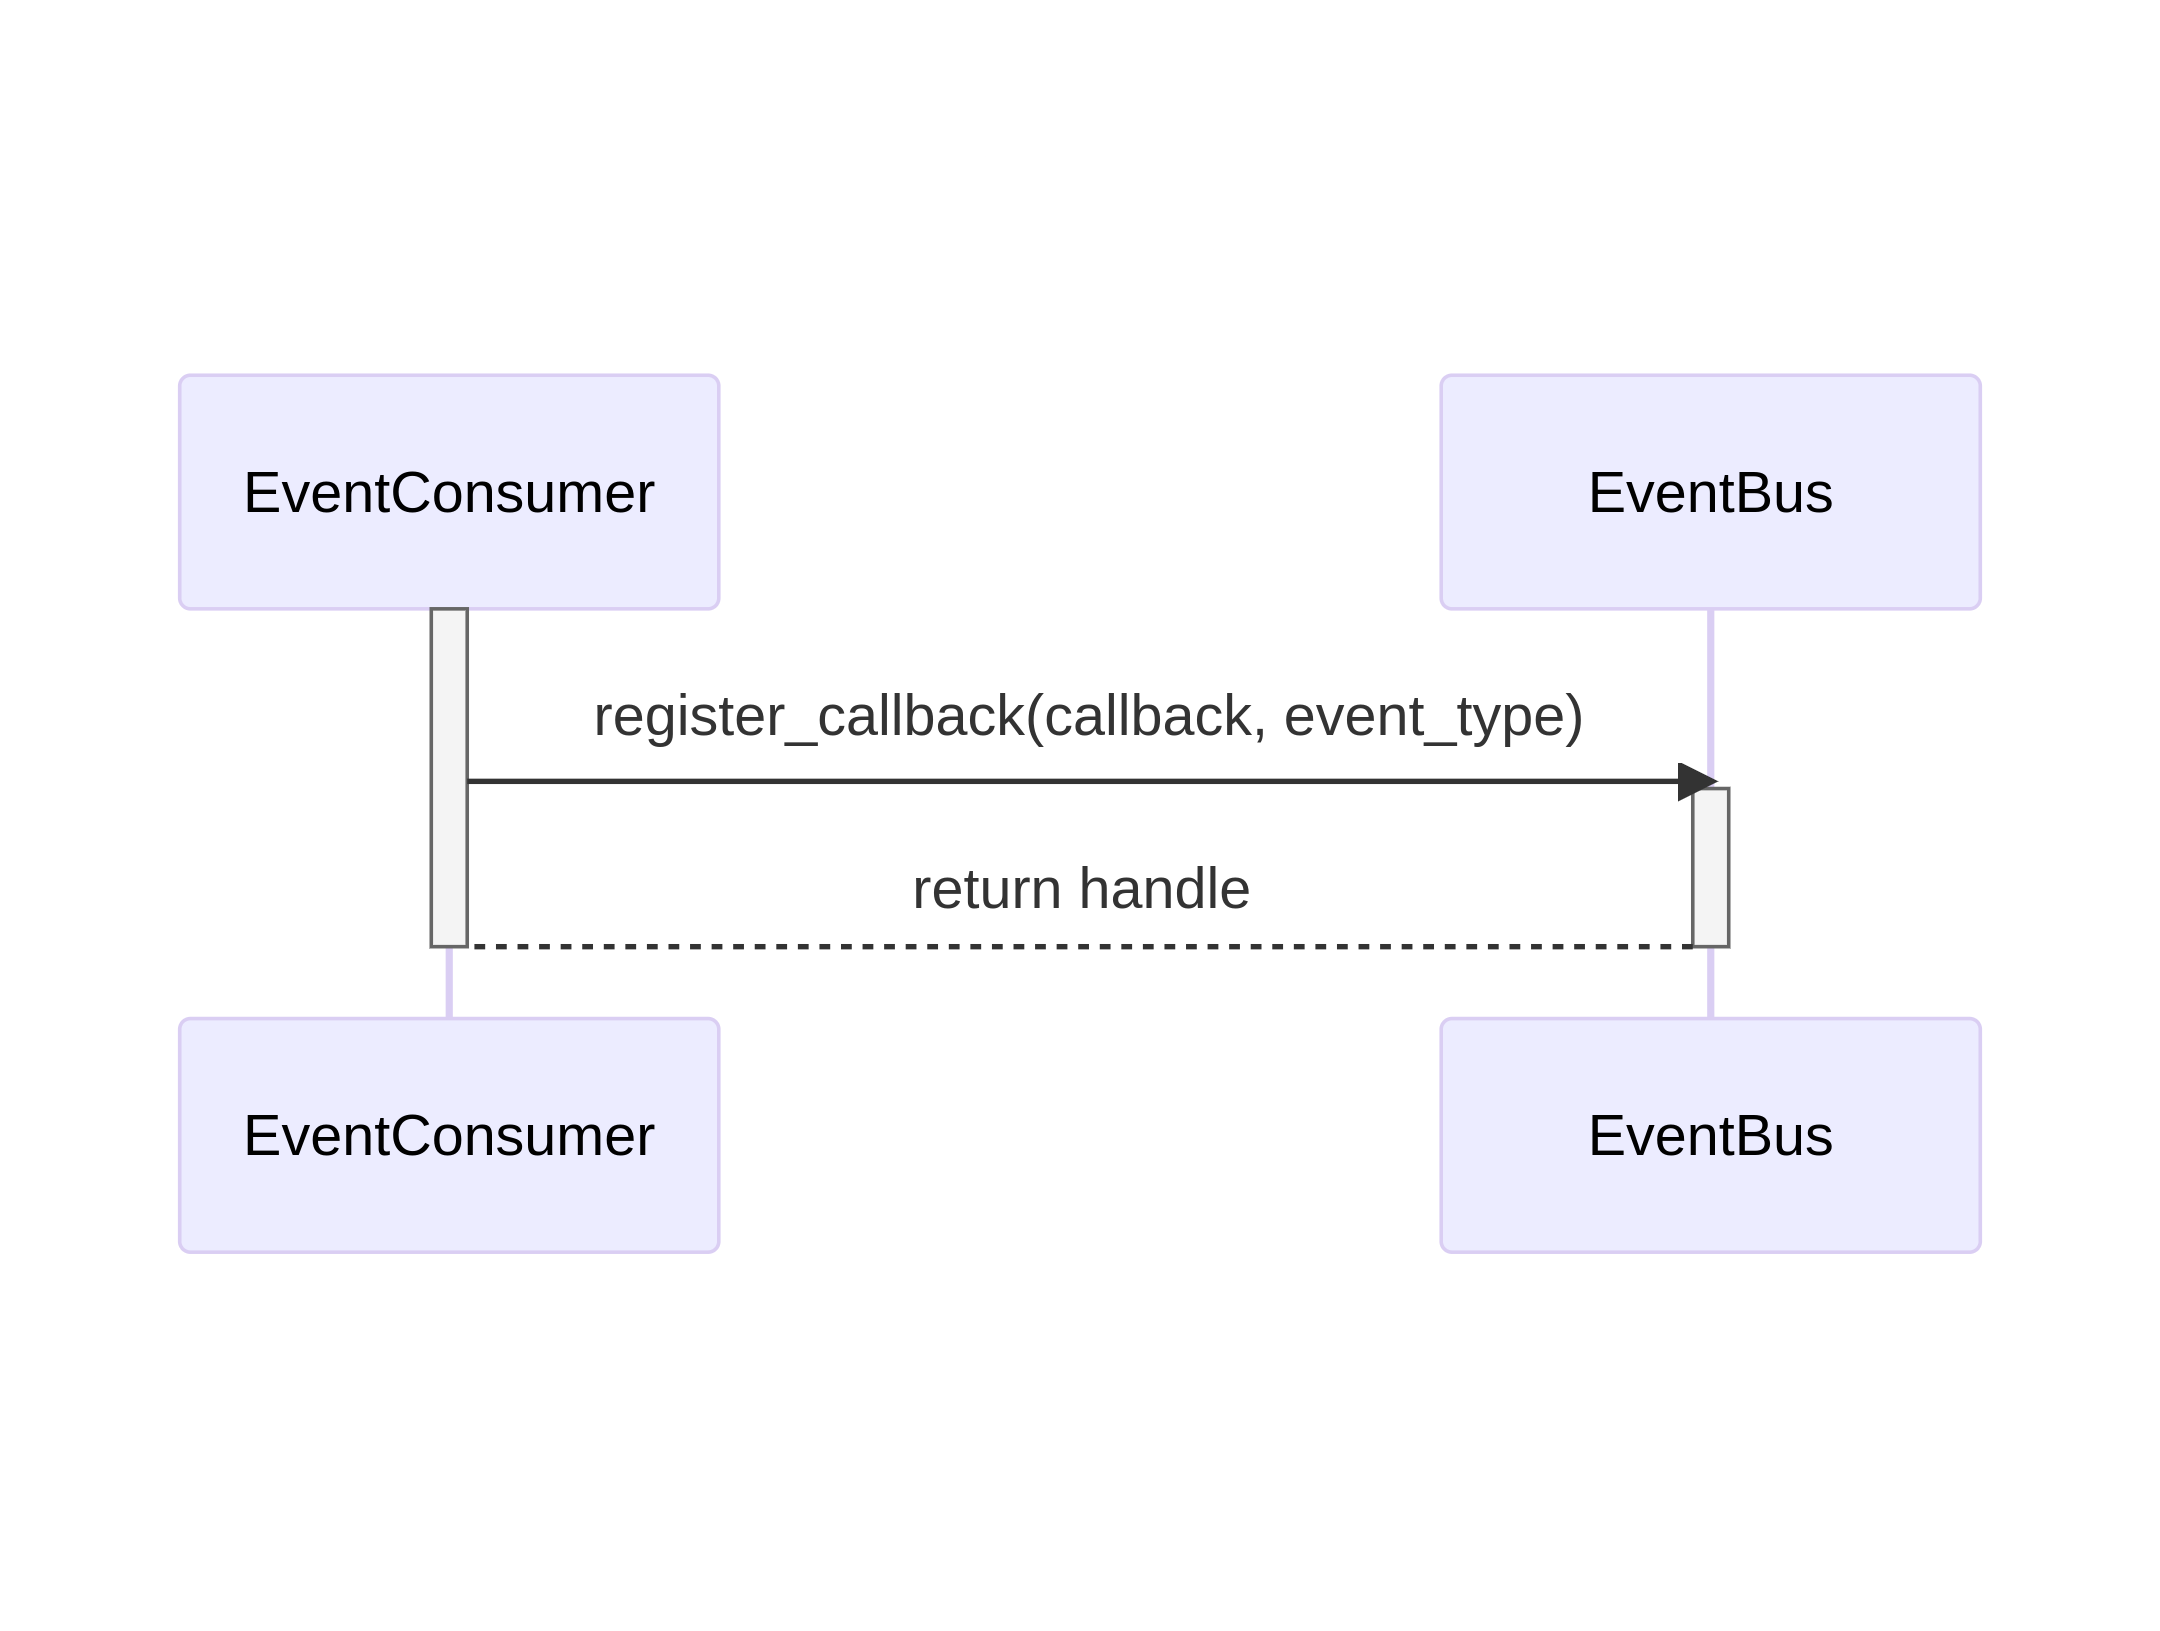
\includegraphics[width=0.75\linewidth]{images/diagrams/eventbus-register-seq.png}
	\caption{Sequenzdiagramm der Registrierung eines Empfängers beim Eventbus.}
	\label{fig:eventbus-register-seq}
\end{figure}

\begin{figure}[!ht]
	\centering
	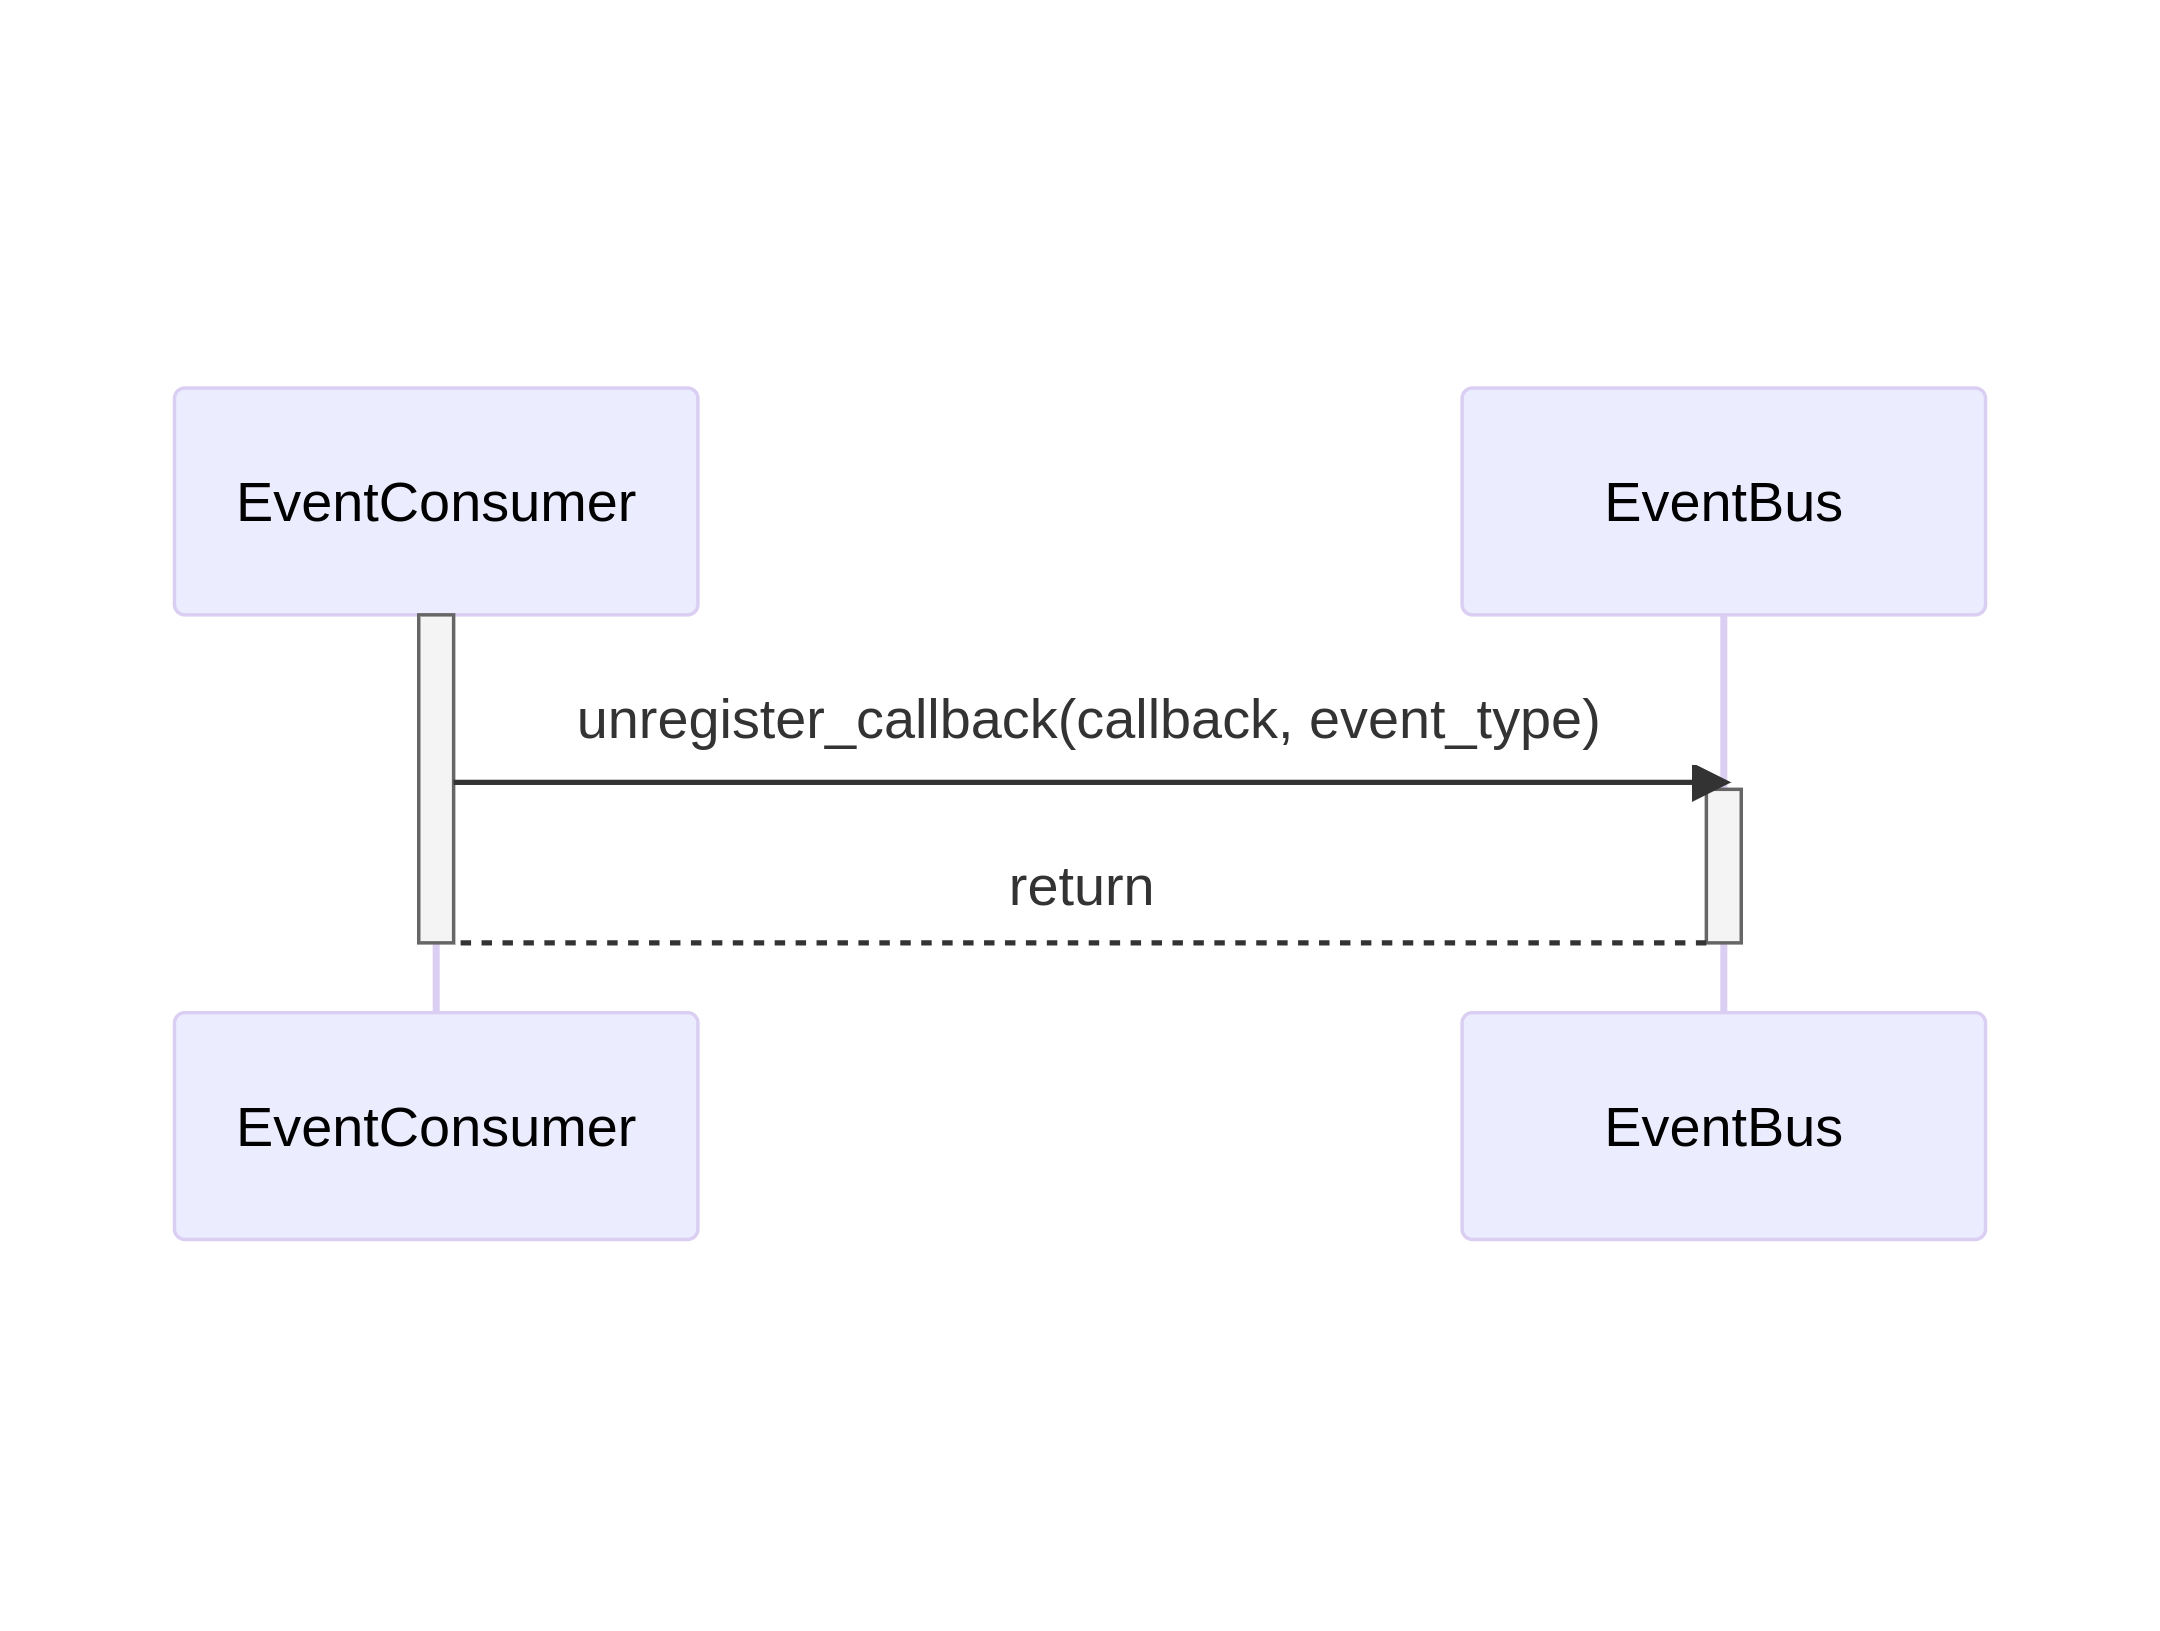
\includegraphics[width=0.75\linewidth]{images/diagrams/eventbus-unregister-seq.png}
	\caption{Sequenzdiagramm der Deregistrierung eines Empfängers beim Eventbus.}
	\label{fig:eventbus-unregister-seq}
\end{figure}

Die Implementierung des Eventbus erfolgte vergleichsweise spät im Projektverlauf. Die Codebasis war bereits entsprechend groß, was uns vor die Herausforderung stellte, wie der Eventbus am besten zu integrieren sei. Auch spielte die Zeitplanung dabei eine Rolle.\\
\\
Da der \emph{Logger} \cite{reisener_entwurf_2023} bereits die Aufgabe übernahm, Ereignisse zu sammeln, lag der Gedanke nahe, ihn entsprechend zu erweitern. Diese Möglichkeit ist im Folgenden unter ''Variante 1 - Erweiterung des \emph{Loggers}'' beschrieben.\\
\\
Da diese Variante gewisse Nachteile mit sich bringt, wird unter ''Variante 2 - Eigenständige Komponente'' eine architektonisch sauberere Lösung vorgestellt. Für diese zweite Lösung haben wir uns aus unten genannten Gründen letztendlich entschieden.

\subsubsection*{Variante 1 - Erweiterung des \emph{Loggers}}

Bei dieser Variante wird das System des \emph{Loggers} erweitert, um die Aufgaben des Eventbus zu übernehmen. Wie \autoref{fig:eventbus-v1-class} zeigt, erstellt der \emph{Logger} für jedes Ereignis ein \code{LogEntry}-Objekt, welches in die Datenbank geschrieben wird. Das \code{LogEntry}-Objekt erbt daher von \code{BaseModel} und besitzt eine \code{save}-Methode, welche bei Erzeugung des Objektes stets ausgeführt wird. Darin wird der Eventbus benachrichtigt, welcher dann die registrierten Empfänger über das neue Ereignis informiert. Die Empfänger realisieren dazu die \code{IEventConsumer}-Schnittstelle, welche eine \code{on\_event}-Methode zur Ereignisbehandlung und ein \code{event\_handle}-Attribut zur Referenzierung der Registrierung beim \code{EventBus} bereitstellt. Die registrierten \emph{Callbacks} werden im Attribut \code{callbacks} gehalten. Es handelt sich dabei um eine Liste von 2-Tupeln, welche das \emph{Callback} und den Ereignistyp enthalten. Ein \emph{Callback} nimmt dabei ein \code{LogEntry}-Objekt entgegen und hat keinen Rückgabewert.

\begin{figure}[!ht]
	\centering
	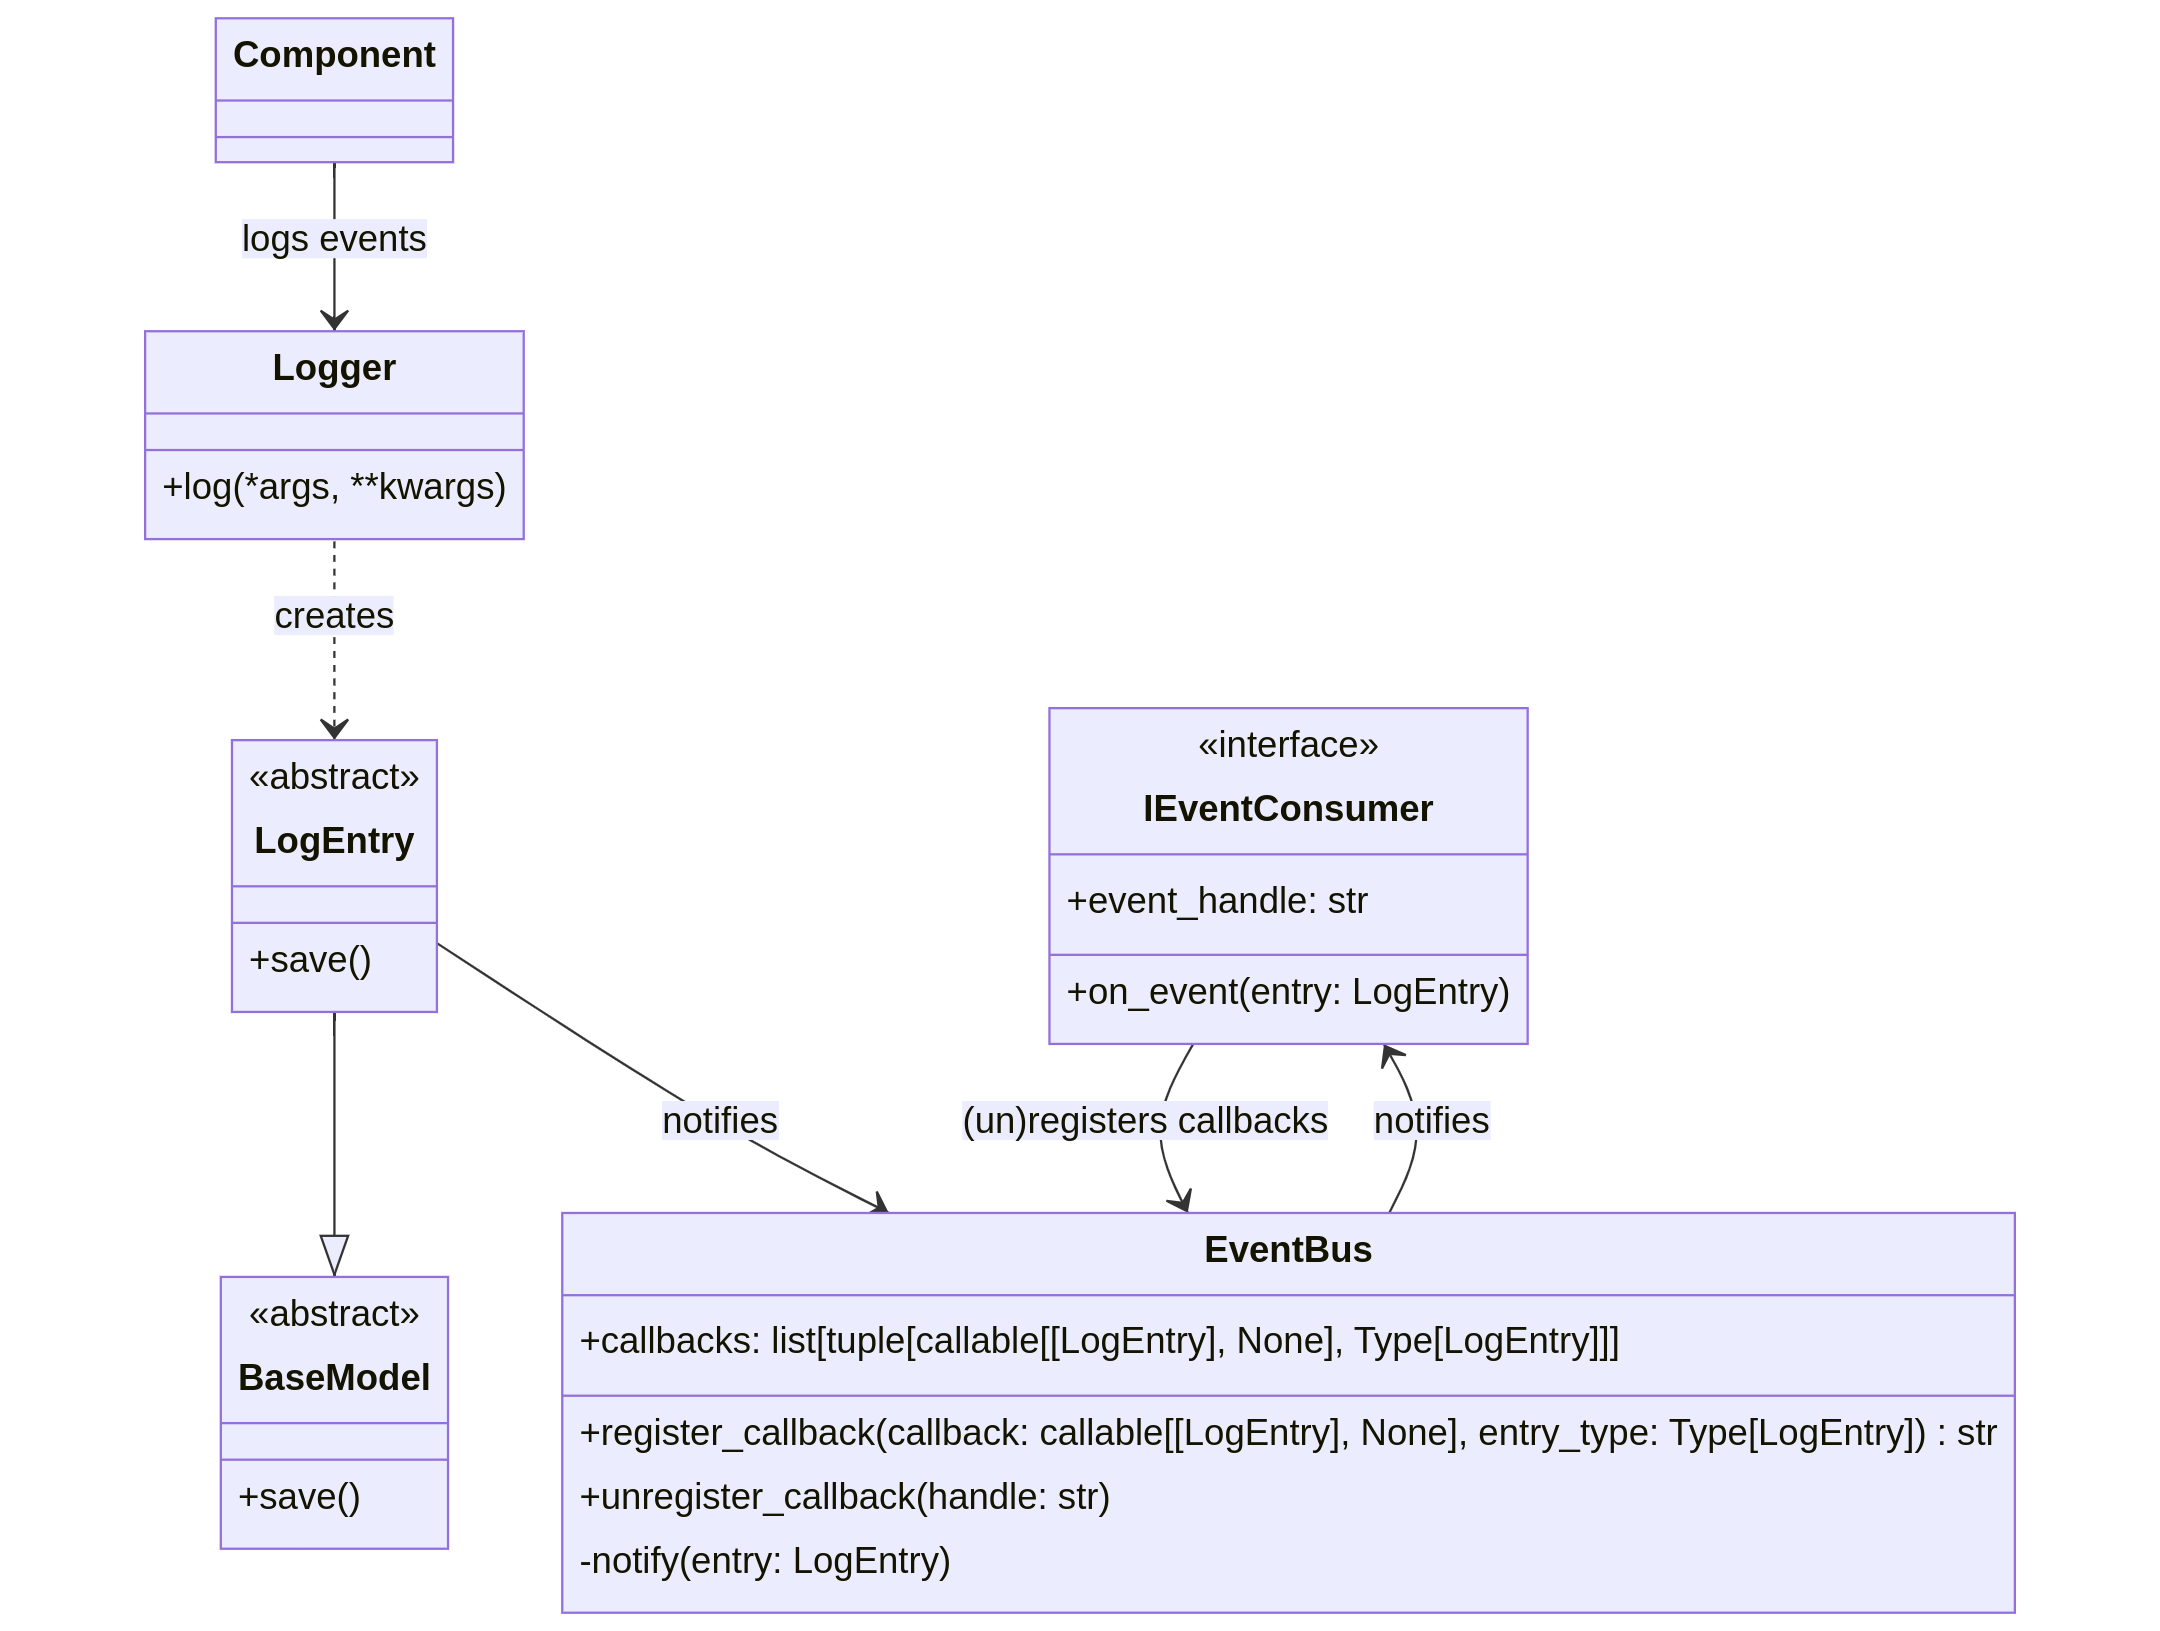
\includegraphics[width=1.0\linewidth]{images/diagrams/eventbus-v1-class.png}
	\caption{Klassendiagramm der ersten Variante des Eventbus.}
	\label{fig:eventbus-v1-class}
\end{figure}

\autoref{fig:eventbus-v1-seq} zeigt den Vorgang der Meldung eines Ereignisses an den \emph{Logger} bis hin zur Benachrichtigung der abhängigen Empfänger. Eine Komponenten (\code{Component}) sendet ein Ereignis durch Aufruf von \code{log} an den \code{Logger} (1). Dieser erzeugt durch \code{create} ein \code{LogEntry}-Objekt (2) und ruft dessen \code{save}-Methode auf (3). Diese benachrichtigt den Eventbus durch Senden von \code{notify} und übergibt dabei das \code{LogEntry}-Objekt selbst (4). Der Eventbus iteriert über die Liste der registrierten \emph{Callbacks} und ruft für jeden Eintrag das \emph{Callback} auf, sofern der Ereignistyp übereinstimmt (5).\\

\begin{figure}[!ht]
	\centering
	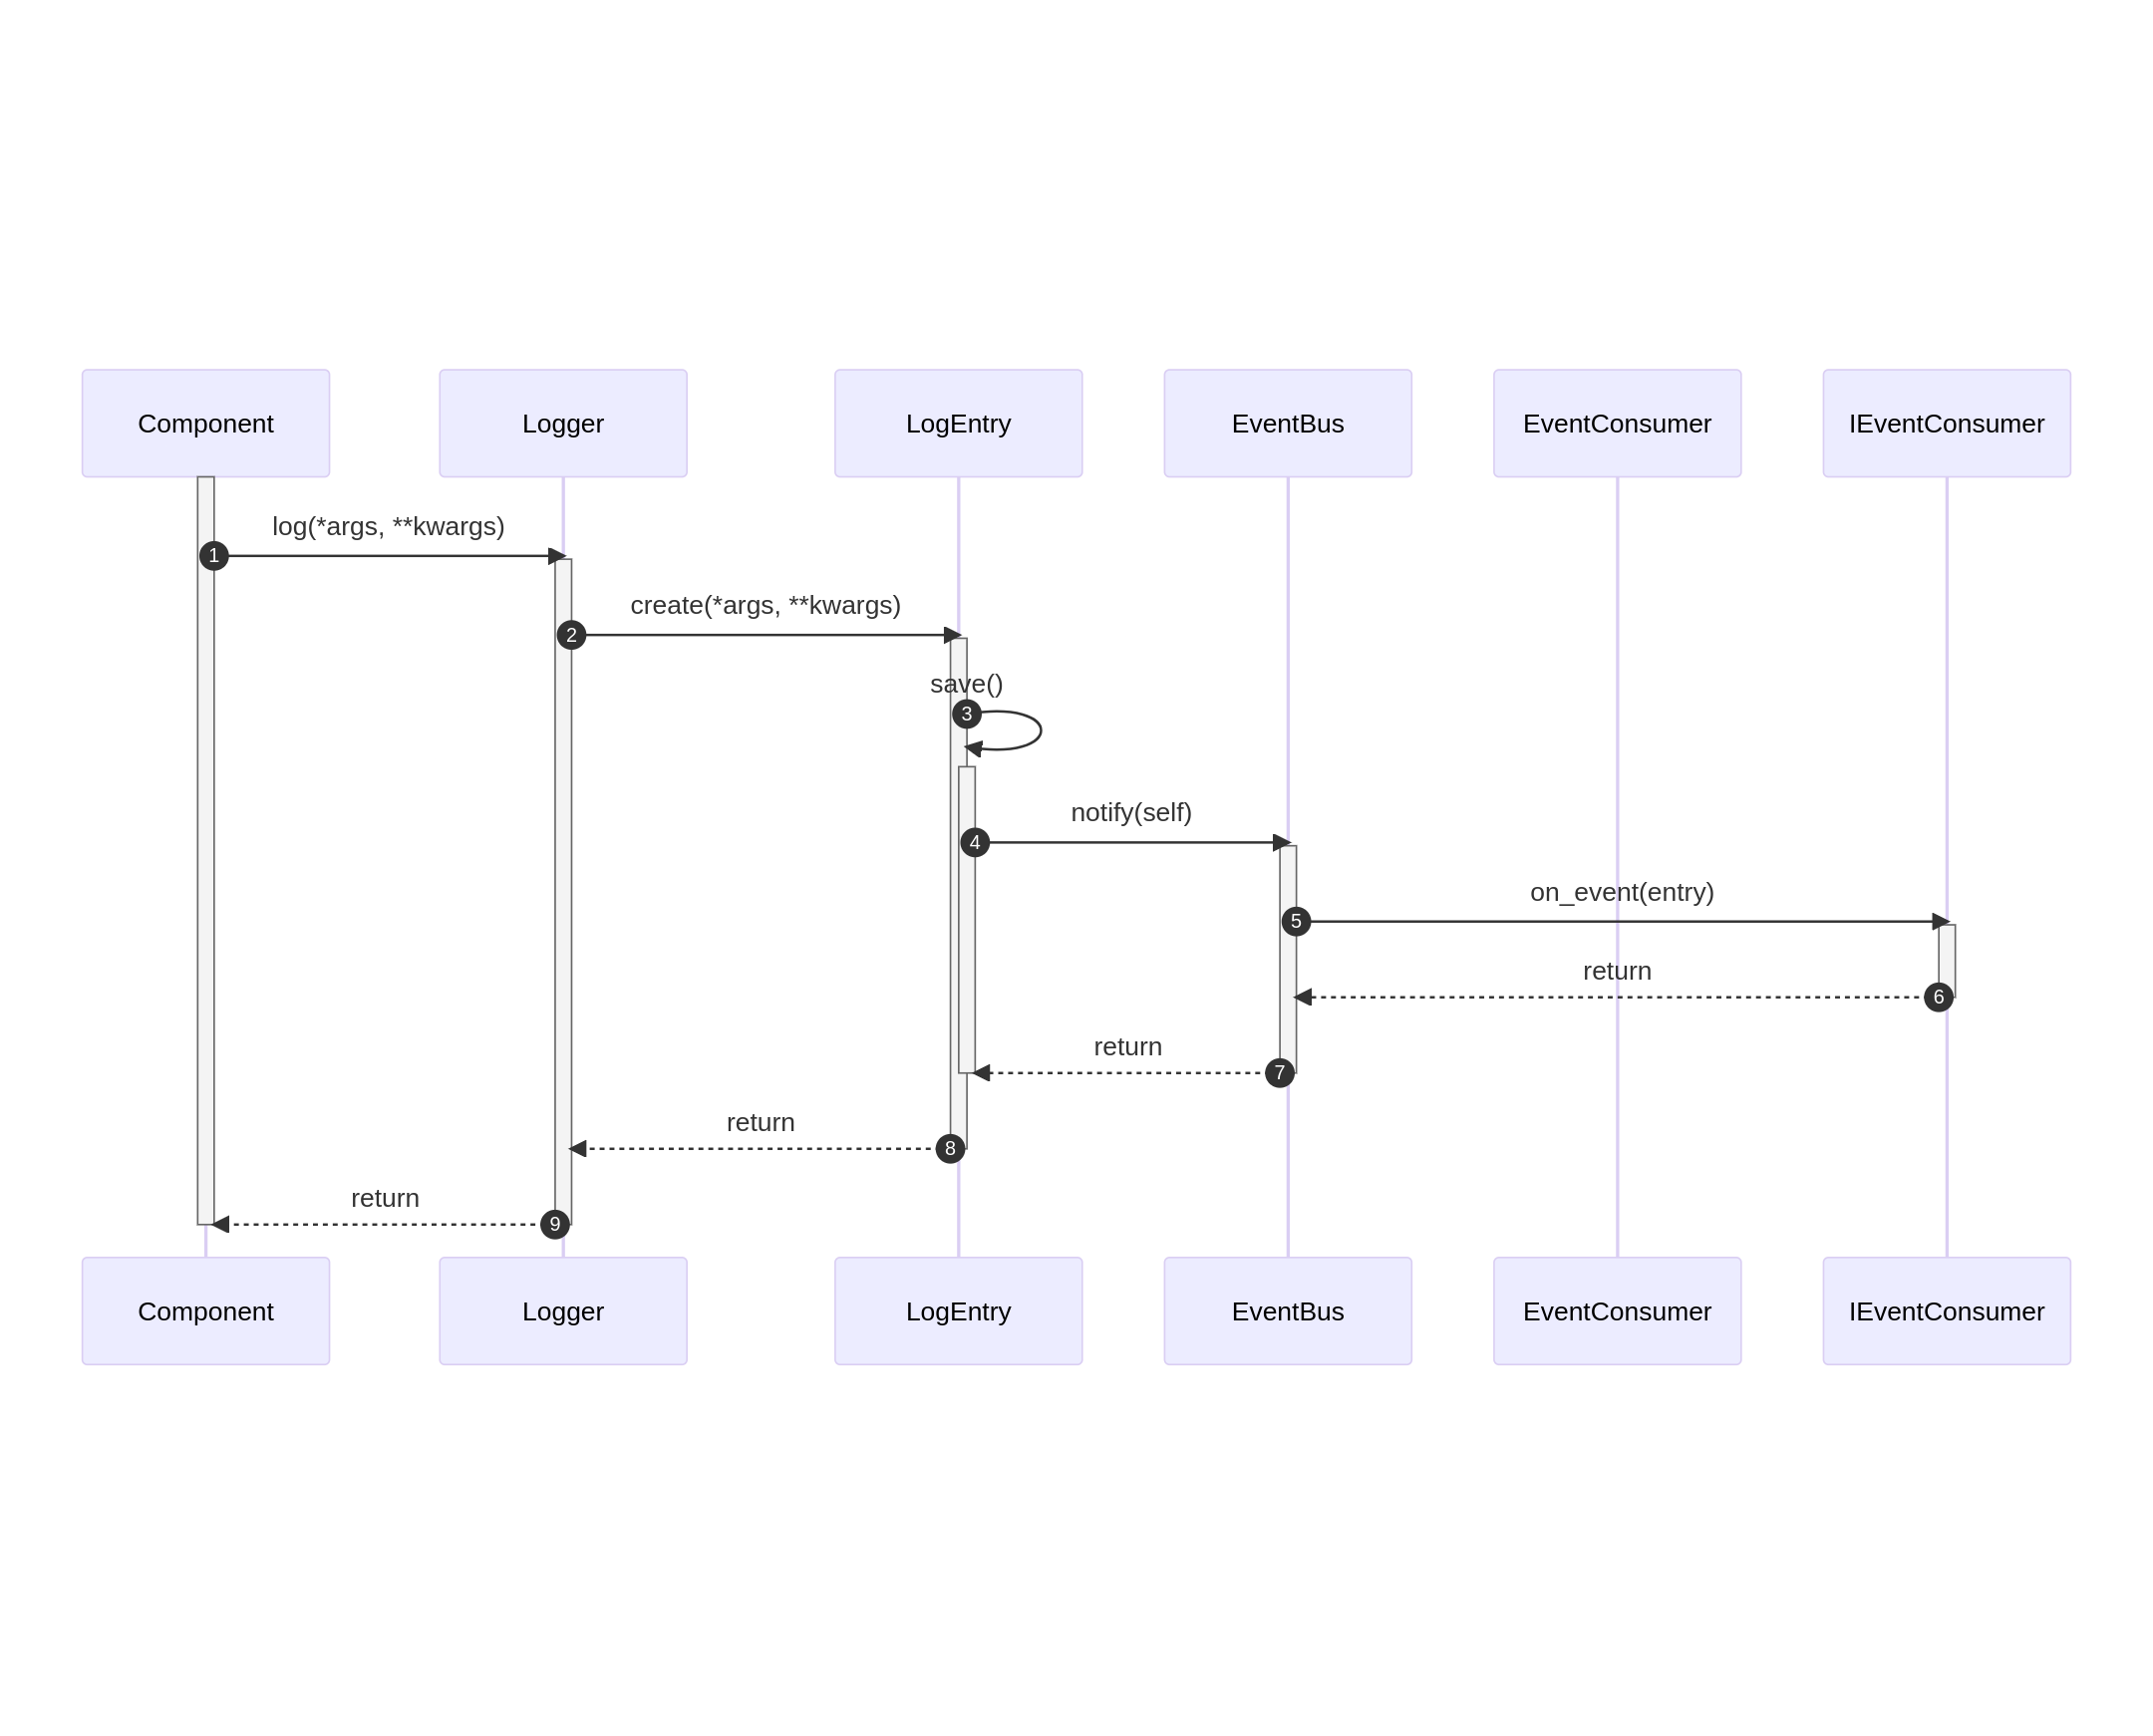
\includegraphics[width=1.0\linewidth]{images/diagrams/eventbus-v1-seq.png}
	\caption{Sequenzdiagramm der ersten Variante des Eventbus.}
	\label{fig:eventbus-v1-seq}
\end{figure}

Der Vorteil dieser Variante ist die einfache Integration in das bestehende System. Die Änderungen am bestehenden Quelltext sind gering. Damit kann die Implementierung des Eventbus schnell erfolgen, was einen positiven Einfluss auf die Zeitplanung hat. Nachteilhaft ist jedoch, dass das \emph{Logging}-System nun auch Teilaufgaben des Eventbus übernimmt. Dies widerspricht dem Prinzip der \emph{Single Responsibility}\footnote{Eine Komponente, Klasse oder Funktion soll nur ein Konzept implementieren oder nur eine Aufgabe erledigen.} und kann zu einer unübersichtlichen Codebasis führen.

\subsubsection*{Variante 2 - Eigenständige Komponente}

Bei dieser Variante wird der Eventbus als eigenständige Komponente implementiert. \autoref{fig:eventbus-v2-class} zeigt das Klassendiagramm. Jede Komponente hält nun eine Referenz auf den Eventbus, um sich als Empfänger registrieren zu können. Die Registrierung und Deregistrierung, sowie die Verwaltung der registrieren \emph{Callbacks} erfolgt wie bei der ''Erweiterung des \emph{Loggers}''. Der Unterschied besteht darin, dass die Ereignisse nun nicht mehr durch \code{LogEntry}-Objekte, sondern durch \code{Event}-Objekte repräsentiert werden. Komponenten benachrichtigen hier selbst den \code{EventBus}. Der \emph{Logger} implementiert die \code{IEventConsumer}-Schnittstelle und registriert sich ebenfalls beim Eventbus, um seine Aufgabe erfüllen zu können.

\begin{figure}[!ht]
	\centering
	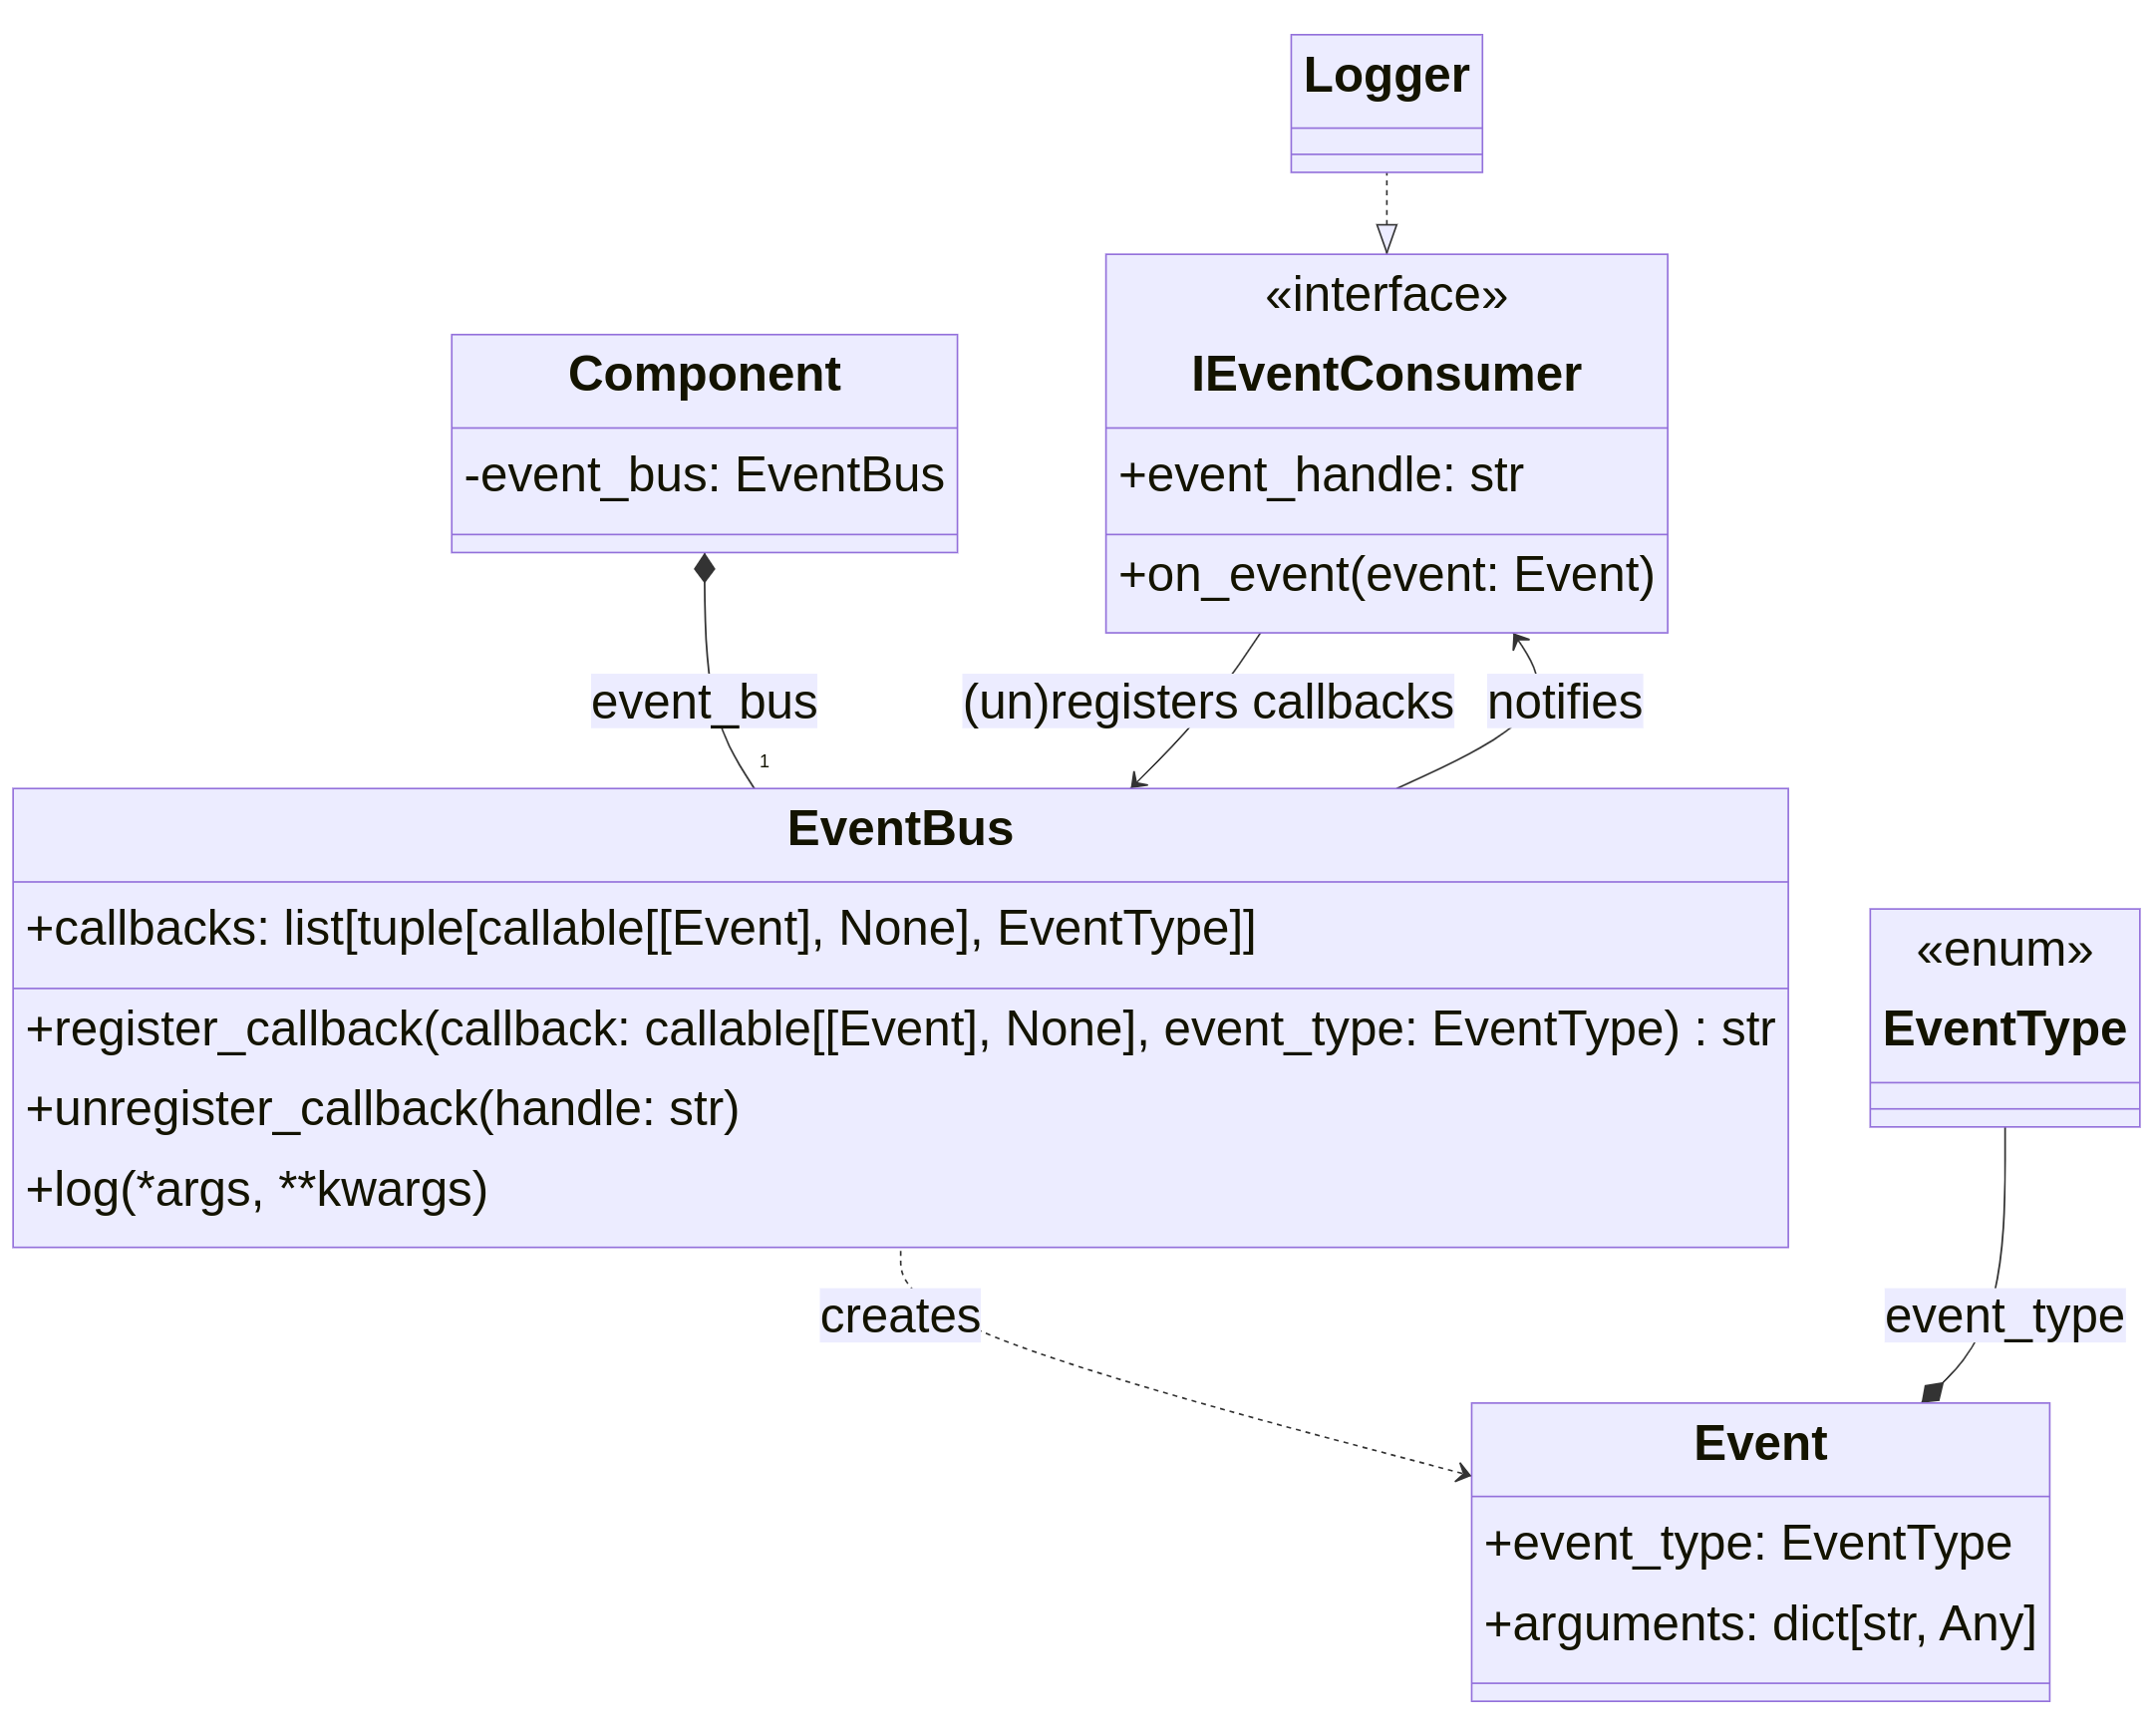
\includegraphics[width=1.0\linewidth]{images/diagrams/eventbus-v2-class.png}
	\caption{Klassendiagramm der zweiten Variante des Eventbus.}
	\label{fig:eventbus-v2-class}
\end{figure}

\autoref{fig:eventbus-v2-seq} zeigt den Ablauf der Meldung eines Ereignisses an den Eventbus. Eine Komponente (\code{Component}) sendet die Parameter eines Ereignisses, durch Aufruf von \code{log}, an den \code{EventBus} (1). Dieser instanziiert ein \code{Event}-Objekt mit den übergebenen Parametern (2). Anschließend iteriert er über die Liste der registrierten \emph{Callbacks} und ruft diese auf, sofern der Ereignistyp übereinstimmt (3).

\begin{figure}[!ht]
	\centering
	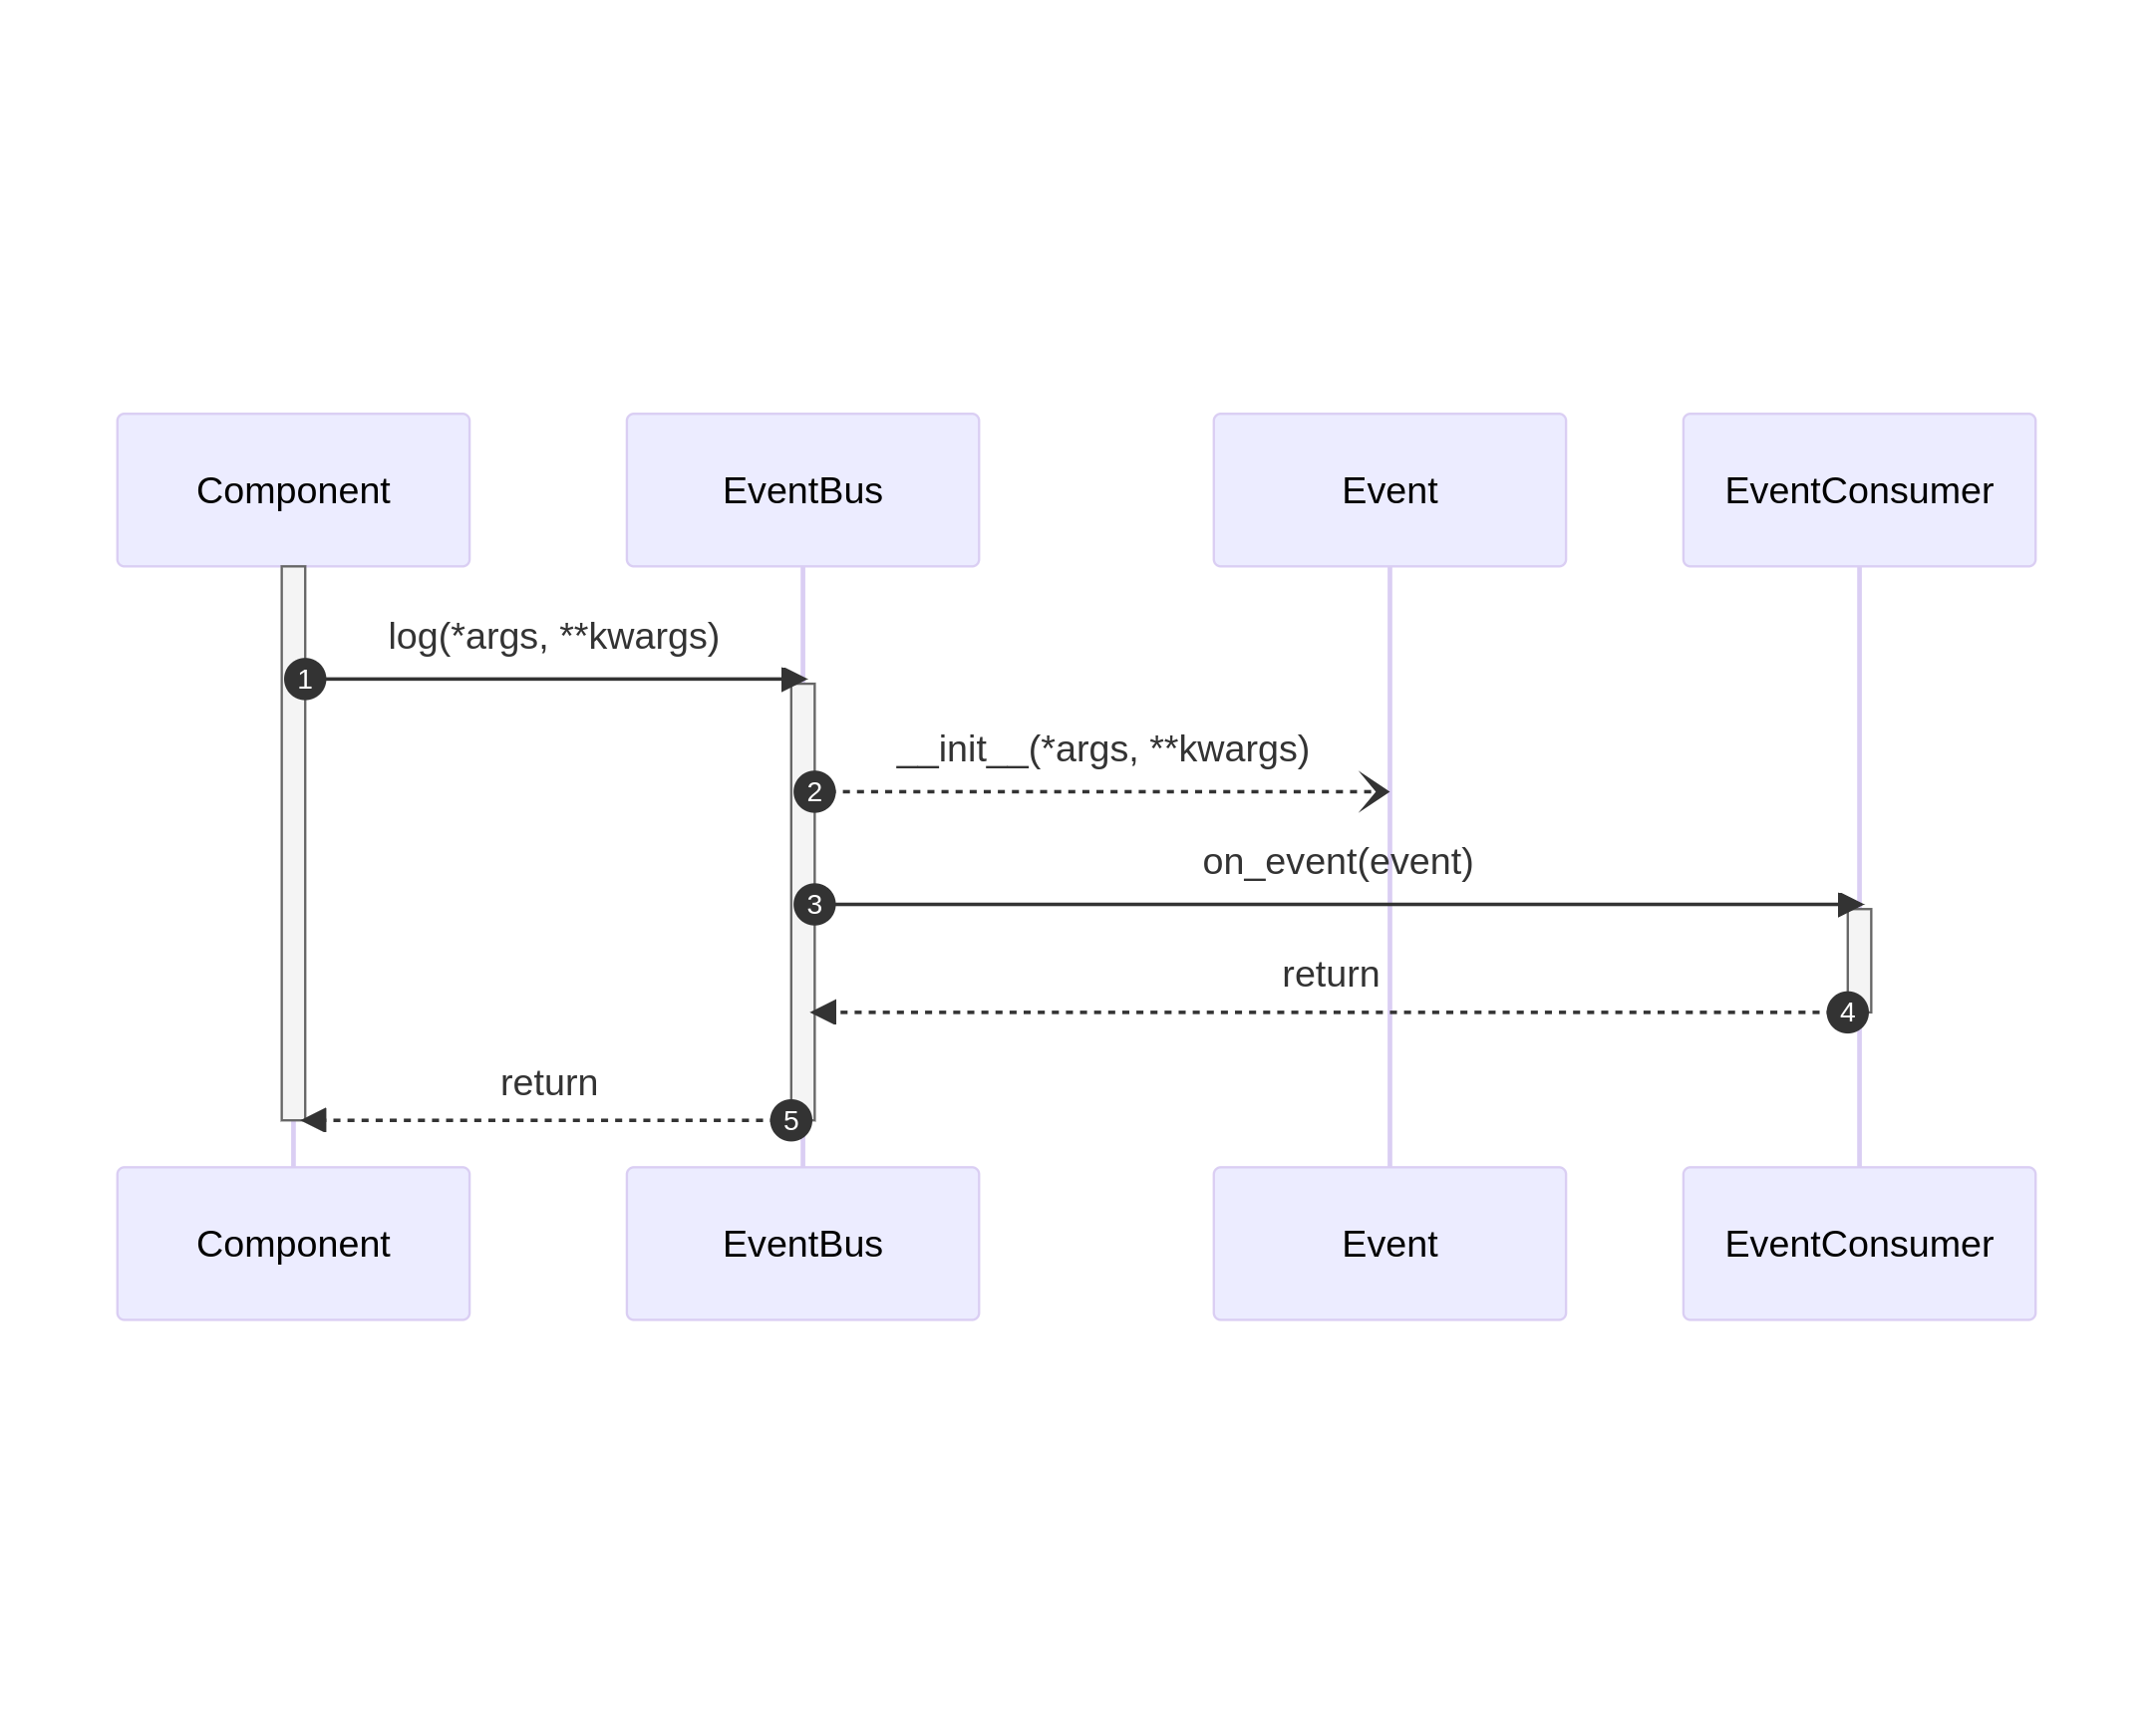
\includegraphics[width=1.0\linewidth]{images/diagrams/eventbus-v2-seq.png}
	\caption{Sequenzdiagramm der zweiten Variante des Eventbus.}
	\label{fig:eventbus-v2-seq}
\end{figure}

Der Vorteil dieser Variante ist die saubere Trennung der Aufgaben des \emph{Loggers} und des Eventbus und die klare Zuordnung der Verantwortlichkeiten. Dafür ist die Implementierung aufwändiger, da mehr Änderungen am bestehenden Quelltext notwendig sind. Das bezieht sich vor allem auf den Umbau des \emph{Loggers}, welcher mit \code{Event}-Objekten statt mit direkt übergebenen Argumenten arbeiten muss. Trotz des Mehraufwandes haben wir uns letztendlich zugunsten der Codequalität für diese Variante entschieden.\\
\\
Eine Verwendung findet der Eventbus im aktuellen System nicht. Aus Zeitgründen wurder der Eventbus zwar implementiert, jedch nicht mehr verwendet. Mögliche Verwendungensind im Ausblick dieser Arbeit beschrieben.